\documentclass{article}
\usepackage[a4paper, total={6in, 8in}]{geometry}
\usepackage{amsmath}
\usepackage{setspace}
\usepackage{xcolor}
\definecolor{DarkRed}{rgb}{0.7725490196,0.05490196078,0.12549019607} % new TU red
\usepackage{courier}
\usepackage[english]{babel}				% \usepackage[ngerman]{babel}
\selectlanguage{english}				% \selectlanguage{ngerman}
\usepackage[T1]{fontenc}
\usepackage[utf8]{inputenc}				% can use native umlauts
\usepackage[babel,english=american]{csquotes}	% provides \enquote{Blupp} => "`Blupp"'
\usepackage{textcomp} 
\makeatletter	
\usepackage{units}		
\usepackage{graphicx}
\usepackage{eso-pic}					% needed for the full-face titlepage
\usepackage{indentfirst}

\begin{document}
\begin{titlepage}
	\AddToShipoutPicture*{
		\put(0,0){
			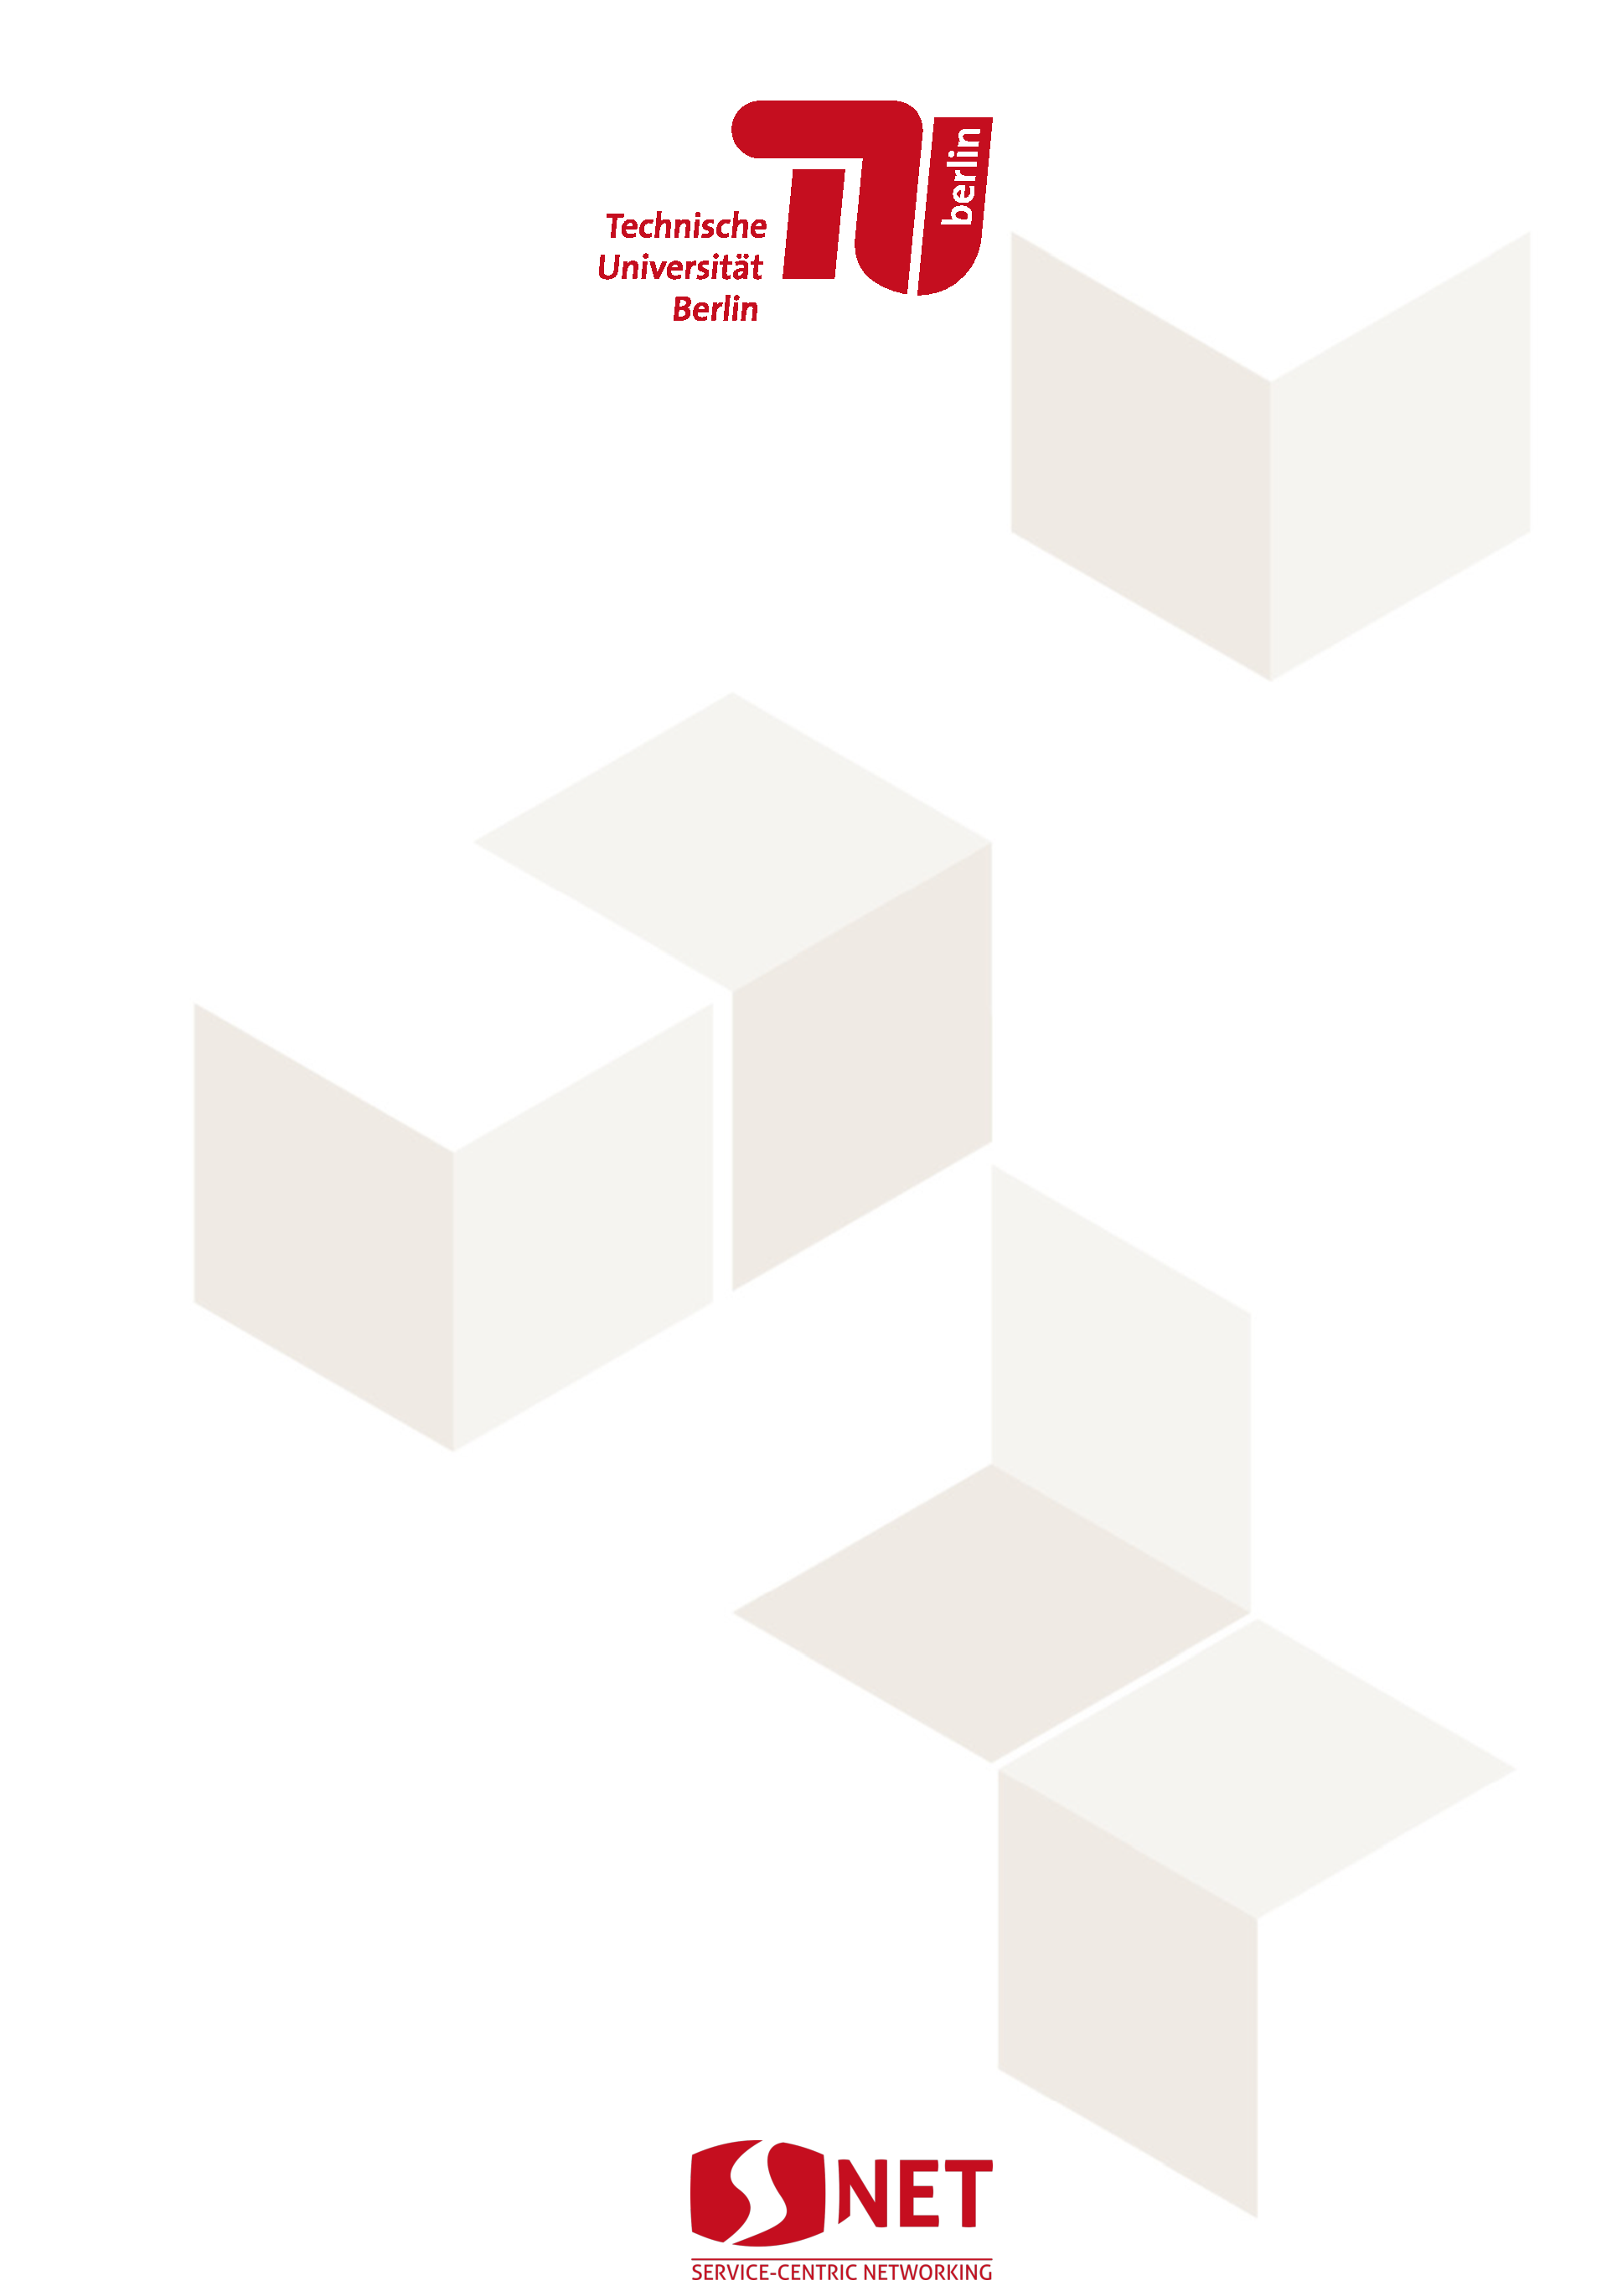
\includegraphics[width=\paperwidth,height=\paperheight,keepaspectratio=false]{images/snet/titlepage.pdf}
		}
	}
	\strut
	\hfill
	\begin{center}
	\vspace{1cm}
		\Huge
		\begin{spacing}{.9}
			\textcolor{DarkRed}{\textbf{Extending Secure Data Storage in Decentralized Networks}}\\
		\end{spacing}
		\vspace{0.8cm}
		\large
		by\\
		\vspace{0.8cm}
		\textbf{Youngrak Ryu}\\
		\vspace{0.8cm}
		\textbf{Matriculation Number 380241}\\
		%vspace{2cm}
	 	%A thesis submitted to\\
	 	\vspace{0.5cm}
		Technische Universität Berlin\\
		School IV - Electrical Engineering and Computer Science\\
		Department of Telecommunication Systems\\
		Service-centric Networking\\
		\vspace{0.5cm}
		Master's Thesis Outline\\
		\vspace{2.2cm}
		\today\\
		\vspace{2.0cm}
		\large
		%Supervised by:\\
		%Dr. Axel Küpper\\
		\vspace{1cm}
		supervisor:\\
		%Assistant supervisor:\\
		Dirk Thatmann
		\end{center}
         		%\includegraphics[scale=1.0]{images/watermark.png}
\end{titlepage}

% Clear two pages after the title
%\shipout\null
%\shipout\null


{\huge  \textbf {Data storage in DHTs: A Framework for storing larger data in Kademlia}}\\
\section{State of the Art}
Most legacy network systems are composed as centralized architecture, in which the main system afford services to connected users. When users request any information, the front-end application takes over requests of the user and brings data from the connected server or back-end application. This manner takes advantage of development and management. However, as the growing scale of the system, the centralized network encounters difficulties, e.g., network connection instability, DDoS, storage cost with rising scale, and sensitive data management. In contrast to the centralized network system, the decentralized network system has become a big trend to avoid the disadvantages of the centralized network. 
Distributed Ledger Technology is one of the decentralized network technologies. It is composed of nodes that verify with the cryptographical identifier, then interconnect using the peer-to-peer network, and transmit data between nodes. The system to avoid data modification uses consensus algorithms for reliable nodes. The decentralized storage to share data uses the distributed file system, e.g., InterPlanetary File System (IPFS),  \cite{IPFS}\cite{benet2014ipfs}, BitTorrent File System (BTFS)\cite{BTFS}, Ethereum Swarm, and BigchainDB. The distributed file systems are characterized by sharing fragmented data as a chunk that is stored in nodes. It relies on distributed hash tables (DHT)\cite{sivaraja2008efficient}, which is a lookup service using key and value or list paired. Using encrypted key DHT can get exact values. With distinguish DHT characters, more use cases are extended (e.g., e-Wallet, Digital Identification, Distributed File System, and Peer-to-Peer file sharing). DHT based P2P system uses some algorithms such as Cord, CAN, Pastry, Tapestry, and Kademlia. Kademlia has a binary tree structure and uses the XOR metric to calculate the distance between nodes. The characteristic of Kademlia is that between nodes communicate using a UDP based transmission. Thus, the current UDP based Kademlia system has a restriction for storing a large amount of data. 

Many different consensus algorithms, DHT, and databases have emerged to meet the challenge of distributed systems.

\section{Scope of the thesis }
The target scenario to be supported is a UDP based Kademlia system\cite{maymounkov2002kademlia}, thus as a DHT to extend the ability to store data packets larger than the MTU (1500bytes) distributed\cite{ietf-intarea-frag-fragile-17}. However, UDP has no transmission control, that lost packets cannot be re-requested, so packet fragmentation, i.e., splitting data across packets, becomes a problems\cite{rfc791}\cite{rfc815}. 
In this thesis, a protocol and framework will be developed to help store large amounts of data in a UDP-based DHT. To enable secure decentralized data storage requires comparison and analyzation between other systems. Furthermore, I would like to develop a framework with research findings. 

\section{Problem}
MTU has the limitation of the size of a single packet, 1500bytes. When the client transfers to another node data such as an image file over 1500bytes, the transmission use Packet Fragmentation, which splits packets into smaller pieces, and then fragmented packets are sending to avoid MTU. Fragmented packets are reassembled at the received host. However, the packet fragmentation can occur technical problems, which are packet filtering at the Firewall or NAT router, fragmented packets can be lost in the transmission. UDP cannot control the transmission, so the node cannot guarantee received data. Thus, to complete transmission, the node should keep sending data. Therefore the latency can increase with the retransmission of data. With the data loss problem, the interconnected nodes have trouble synchronizing data. The nodes cannot trust each other, and the reliability problem may arise from unsynchronized data.
In Kademlia DHT, participated nodes are identified by number or node ID, which is composed as file hash or keywords. In a security aspect, file hash or keyword for the identification has a lack of functionality and security. It is necessary to find a way to identify participated nodes.
The system is feasibly designed to interconnect between various platforms, e.g., PC, smartphone, and IoT. The framework will be developed into cross-compile based. Most IoTs are limited environment and offer minimized resource. Therefore the framework has to be compressed and not to be heavy.

\section{Approach}

The framework will be developed to solve issues problems. The overall approach in this thesis is to enable the extended DHT system to store data packets larger than MTU. The framework will apply UDP based Kademlia DHT. As improve the transmission ability of the lager data packet, the problem may solve using two different ways. First, Kademlia DHT should be able to transfer a larger amount of data. The prototype may use other ethernet frames or network protocols to extend the possibility of larger data transfer. The other way is using checksum functionality. The prototype should verify the integrity of the transferred data. UDP, which is a message-oriented protocol, does not support packet fragmentation and error correction. Therefore it has no reordering or retransmitting mechanism. The framework needs checksum functionality. The data checksum will be applied to avoid packet loss. The prototype will be improved to increase the amount of data transfer and to reduce transmission error. Furthermore, the developed framework would like to make a trial of using IPFS and BTFS, and then with the findings, the prototype will be applied. Nodes make a connection via the P2P tunnel to enable data storage in decentralized networks. As establish P2P, between nodes have to verify credentials. Self-Sovereign Identity (SSI)\cite{tobin2016inevitable} will be applied and uses the Decentralized identifier (DID)\cite{sabadello2018introduction}. The framework will also implement SSI using DID. The prototype will be developed by ANSI C language for supporting extending various platforms such as IoT devices. For testbed, an environment will be configured using Docker-composed. Virtual nodes will be implemented using Docker-compose, and then the prototype will make tests on the environment.


\section{Challenge}
The most critical challenge is the efficient data transmission between nodes, which are the usability of larger data packet transmission and transmission control. As develop larger data transmission, the framework should control data transmission, e.g., compression, propagation speed, message latency, fragmentation. If as possible, the prototype can combine an extending Kademlia DHT using other protocols. This solution may help the limitation problem of packet size. The decentralized network can extend transmittable feasible data types, e.g., image, the large amount of the dataset, and music, over the existing limitation.

Furthermore, nodes of different types, such as heterogeneous devices, should be feasible to connect with each other. The growth of IoT would be the leading node platform in the decentralized network. Numerous IoT device nodes will deploy on the network, thus developing the cross-compiling framework is a significant assignment. For reaching the requirement framework will be Ansi C implementation and composed scale for using limited IoT resources as well.


\section{Evaluation}
The completely developed prototype will be evaluated by demanded procedures. The prototype will make an interoperability test. To evaluate the prototype progresses a simulation of transmission mass data distribution. In the simulation, the between nodes will read or write data through the findings that can be analyzed as pros and cons. The evaluation should analyze the comparison of the implemented prototype between other systems such as IPFS, BTFS, and standard Kademlia by measurement of transmission rate, error rate, latency, propagation speed, and reliability. Through the user test, the developed system can verify more issues. Discovered new challenges or developable problems can be further work.

\section{Schedule}

\begin{table} [h]
	\centering
	%\begin{flushleft}
	\begin{tabular}{ p{2cm} p{13cm} }
	%\raggedleft
		$\bullet$ 1/2 month & Research of decentralized network systems and related work \\
		$\bullet$ 1/2 month & Design the prototype\\
		$\bullet$ 1/2 month & Implement the network and other systems \\
		$\bullet$ 1 month & Develop and implement the prototype\\
		$\bullet$ 1 month & Improve the developed prototype\\
		$\bullet$ 1/2 month & Simulation and evaluation \\
		$\bullet$ 2 month & Write thesis \\
	\end{tabular}
	%\end{flushleft}
\end{table}

\newpage

\bibliographystyle{IEEEtran}
\bibliography{bibliography.bib}
\end{document}

